\documentclass{beamer}

\mode<presentation> {

%\usetheme{default}
%\usetheme{AnnArbor}
%\usetheme{Antibes}
%\usetheme{Bergen}
%\usetheme{Berkeley}
%\usetheme{Berlin}
%\usetheme{Boadilla}
%\usetheme{CambridgeUS}
%\usetheme{Copenhagen}
%\usetheme{Darmstadt}
%\usetheme{Dresden}
%\usetheme{Frankfurt}
%\usetheme{Goettingen}
%\usetheme{Hannover}
%\usetheme{Ilmenau}
%\usetheme{JuanLesPins}
%\usetheme{Luebeck}
\usetheme{Madrid}
%\usetheme{Malmoe}
%\usetheme{Marburg}
%\usetheme{Montpellier}
%\usetheme{PaloAlto}
%\usetheme{Pittsburgh}
%\usetheme{Rochester}
%\usetheme{Singapore}
%\usetheme{Szeged}
%\usetheme{Warsaw}


%\usecolortheme{albatross}
%\usecolortheme{beaver}
%\usecolortheme{beetle}
%\usecolortheme{crane}
%\usecolortheme{dolphin}
%\usecolortheme{dove}
%\usecolortheme{fly}
%\usecolortheme{lily}
%\usecolortheme{orchid}
%\usecolortheme{rose}
%\usecolortheme{seagull}
%\usecolortheme{seahorse}
%\usecolortheme{whale}
%\usecolortheme{wolverine}

%\setbeamertemplate{footline} % To remove the footer line in all slides uncomment this line
%\setbeamertemplate{footline}[page number] % To replace the footer line in all slides with a simple slide count uncomment this line

%\setbeamertemplate{navigation symbols}{} % To remove the navigation symbols from the bottom of all slides uncomment this line
}

\usepackage{graphicx} % Allows including images
\usepackage{booktabs} % Allows the use of \toprule, \midrule and \bottomrule in tables
\usepackage{amsfonts}
\usepackage{mathrsfs}
\usepackage{amsmath,amssymb,graphicx}

%----------------------------------------------------------------------------------------
%	TITLE PAGE
%----------------------------------------------------------------------------------------

\title["6.1"]{6.1: Statistics And Their Distributions} % The short title appears at the bottom of every slide, the full title is only on the title page

\author{Taylor} % Your name
\institute[UVA] % Your institution as it will appear on the bottom of every slide, may be shorthand to save space
{
University of Virginia \\ % Your institution for the title page
\medskip
\textit{} % Your email address
}
\date{} % Date, can be changed to a custom date

\begin{document}
%----------------------------------------------------------------------------------------

\begin{frame}
\titlepage 
\end{frame}
%----------------------------------------------------------------------------------------

\begin{frame}
\frametitle{Definitions}

\begin{itemize}
\item Random variables are typically denoted with letters at the end of the alphabet (e.g. X,Y, etc.)
\item Before we observe a sample, the data is random ($X_1 , \ldots X_N$)
\item The observations or data we observe are lower-case ($x_1, \ldots x_n$)
\item for more info see Chapter 3
\end{itemize}

\end{frame}
%----------------------------------------------------------------------------------------

\begin{frame}
\frametitle{Definitions}

\begin{itemize}
\item The same idea applies to functions of the rvs 
\item Example: $f(X_1, \ldots, X_n) = \frac{1}{n}\sum_i X_i$ 
\item if we have the data already it's $f(x_1, \ldots, x_n) = \frac{1}{n}\sum_i x_i$
\item This is what a \textbf{statistic} is: a quantity calculated from sample data.
\item We're usually referring to the random variable (capital letters) because we like to talk about it's distribution/moments etc.
\end{itemize}

\end{frame}
%----------------------------------------------------------------------------------------

\begin{frame}
\frametitle{Examples}

Some very ubiquitous examples:

\begin{itemize}
\item $f(X_1, \ldots, X_n) = \frac{1}{n}\sum_i X_i = \bar{X}$ 
\item $f(X_1, \ldots, X_n) = \frac{1}{n-1}\sum_i (X_i - \bar{X})^2 = S^2$
\item $f(X_1, \ldots, X_n) = max(X_1, \ldots, X_n) = X_{(n)} $
\item $f(X_1, \ldots, X_n) = min(X_1, \ldots, X_n) = X_{(1)} $
\end{itemize}
\end{frame}
%----------------------------------------------------------------------------------------


\begin{frame}
\frametitle{Definitions}
\begin{itemize}
\item Every sample statistic has a probability distribution
\item sometimes it's easy to calculate (e.g. the mean of a bunch of normal random variables)
\item sometimes it's difficult or impossible
\item The probability distribution of a statistic is often called a \textbf{sampling distribution}
\item A note on notation: I'll usually denote general probability distributions with a $p$ or an $f$
%\item Some examples: $p_X(x)$, $p_{\bar{X}}(\bar{x})$, $p_{X_1,\ldots,X_n}(x_1,\ldots,x_n)$
\end{itemize}

\end{frame}
%----------------------------------------------------------------------------------------


\begin{frame}
\frametitle{Definitions}
\begin{itemize}
\item Many analyses assume that the data are being generated from a common probability distribution
\item The most tractable situation is when each data point/rv comes from the same distribution, and no data point affects any other data point 
\item the book calls this a \textbf{random sample} (page 287)
\item I will just say (i.i.d) which stands for \emph{independent and identically distributed}
\item I will denote it like this $\overset{iid}{\sim} $
\item example: $X_1, \ldots, X_n \overset{iid}{\sim} \text{Normal}(\mu,\sigma^2)$
\end{itemize}

\end{frame}
%----------------------------------------------------------------------------------------


\begin{frame}
\frametitle{Example}

Our first example (Example 6.3 on page 290):
\newline

Let $X_1, X_2 \overset{iid}{\sim} \text{Exponential}(\lambda)$. What is the distribution of $T_0 = \sum X_i$? First we'll find it's cumulative distribution function (cdf) $F_{T_0}(t)$; then we'll take the derivative to get the density $f_{T_0}(t)$. Hopefully it'll be a familiar distribution again...


\end{frame}
%----------------------------------------------------------------------------------------


\begin{frame}
\frametitle{Example}

\begin{align*}
F_{T_0}(t) &= P(X_1 + X_2 \le t) \\
&= \iint_{ \{(x_1, x_2) : x_1 + x_2 \le t\} } p(x_1, x_2) dx_1 dx_2 \\
&= \iint_{ \{(x_1, x_2) : x_1 + x_2 \le t\} } p(x_1)p(x_2) dx_1 dx_2 \\
&= \int_0^t \int_0^{t-x_1}\lambda e^{-\lambda x_1}\lambda e^{-\lambda x_2} dx_2 dx_1 \\
&= \int_0^t \lambda e^{-\lambda x_1} \left[ \int_0^{t-x_1}\lambda e^{-\lambda x_2} dx_2 \right] dx_1 \\
&= \int_0^t \lambda e^{-\lambda x_1}  \left[- e^{-\lambda x_2} \right]_0^{t-x_1} dx_1 \\
&= \int_0^t \left( \lambda e^{- \lambda x_1} - \lambda e^{- \lambda t}\right)dx_1 
\end{align*}

\end{frame}
%----------------------------------------------------------------------------------------


\begin{frame}
\frametitle{Example}

\begin{align*}
&= \int_0^t \left( \lambda e^{- \lambda x_1} - \lambda e^{- \lambda t}\right)dx_1 \\
&= \int_0^t \lambda e^{- \lambda x_1}dx_1 - t \lambda e^{- \lambda t} \\
&= \left[-e^{-\lambda x_1} \right]_0^t - t\lambda e ^{- \lambda t} \\
&= 1 - e^{- \lambda t} - \lambda t e^{- \lambda t}
\end{align*}

Now differentiate with respect to $t$ to get the density:
\[
f_{T_0}(t) = \lambda ^2 t \exp(- \lambda t), t > 0
\]

\end{frame}
%----------------------------------------------------------------------------------------


\begin{frame}
\frametitle{Notes}
A couple things:

\begin{itemize}
\item this is a $\text{Gamma}(2, 1/\lambda)$ distribution.
\item Recall that there are a few tricks that make Gamma distributions nice 
\item The distribution of sums of independent random variables is made easier by moment generating functions (we'll talk about these later)
\item make sure you get a feel for this (a lot of the same tricks will reappear later)
\end{itemize}

\end{frame}
%----------------------------------------------------------------------------------------


\begin{frame}
\frametitle{Example}

Extending example 6.3:
\newline

Let $X_1, X_2, \ldots, X_N \overset{iid}{\sim} \text{Exponential}(\lambda)$. What is the distribution of $T_0 = \sum_{i=1}^n X_i$? First we'll find it's cumulative distribution function (cdf) $F_{T_0}(t)$; then we'll take the derivative to get the density $f_{T_0}(t)$. 


\end{frame}

%----------------------------------------------------------------------------------------


\begin{frame}
\frametitle{Example}

\begin{align*}
F_{T_0}(t) &= P\left(\sum_{i=1}^n X_i \le t \right) \\
&= \iint_{ \{(x_1, x_2) : x_1 + x_2 \le t\} } f(x_1, \ldots, x_n) dx_{1:n} \\
&= \int_0^t \int_0^{t - \sum_{i=1}^{1} x_i} \cdots \int_{0}^{t - \sum_{i=1}^{n-1} x_i} f(s_1, \ldots, s_n) ds_n ds_{n-1} \cdots ds_{1} 
\end{align*}


\end{frame}

%----------------------------------------------------------------------------------------


\begin{frame}
\frametitle{Example}

Alternatively, you could use the transformation theorem:
\[
\left[\begin{array}{ccc}
Y_1 \\
Y_2 \\
\vdots \\
Y_n
\end{array}\right] 
=
\left[\begin{array}{ccc}
X_1 \\
X_1 + X_2 \\
\vdots \\
\sum_{i=1}^n X_i
\end{array}\right]
\]
It isn't that bad to get $g(y_1, y_2, \ldots, y_n)$, but it's difficult to integrate out $y_1, y_2, \ldots, y_{n-1}$
\end{frame}


%----------------------------------------------------------------------------------------


\begin{frame}
\frametitle{Definitions}

We can also run simulations to check our derivations. 
\newline

Example: If $X_1, \ldots, X_{100} \overset{iid}{\sim} \text{Normal}(0, 1)$, what does the maximum $X_{(100)}$ follow?

\begin{center}
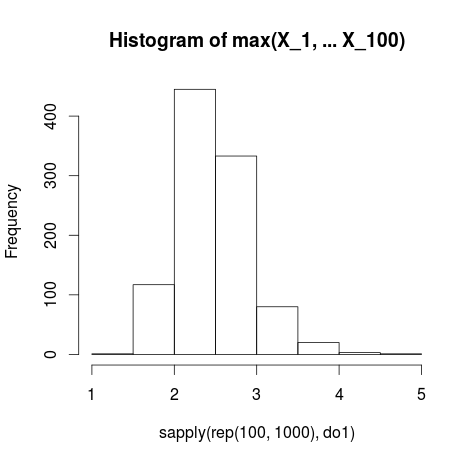
\includegraphics[width=70mm]{/home/t/UVa/all_teaching/summer15_3120/public/slides/6/6.1/sim_hist.png}
\end{center}

\end{frame}
%----------------------------------------------------------------------------------------

\end{document} 